\thispagestyle{toancuabinone}
\pagestyle{toancuabi}
\everymath{\color{toancuabi}}
%\blfootnote{$^1$\color{toancuabi}Đại học Thăng Long.}
\graphicspath{{../toancuabi/pic3/}}
\begingroup
\AddToShipoutPicture*{\put(0,616){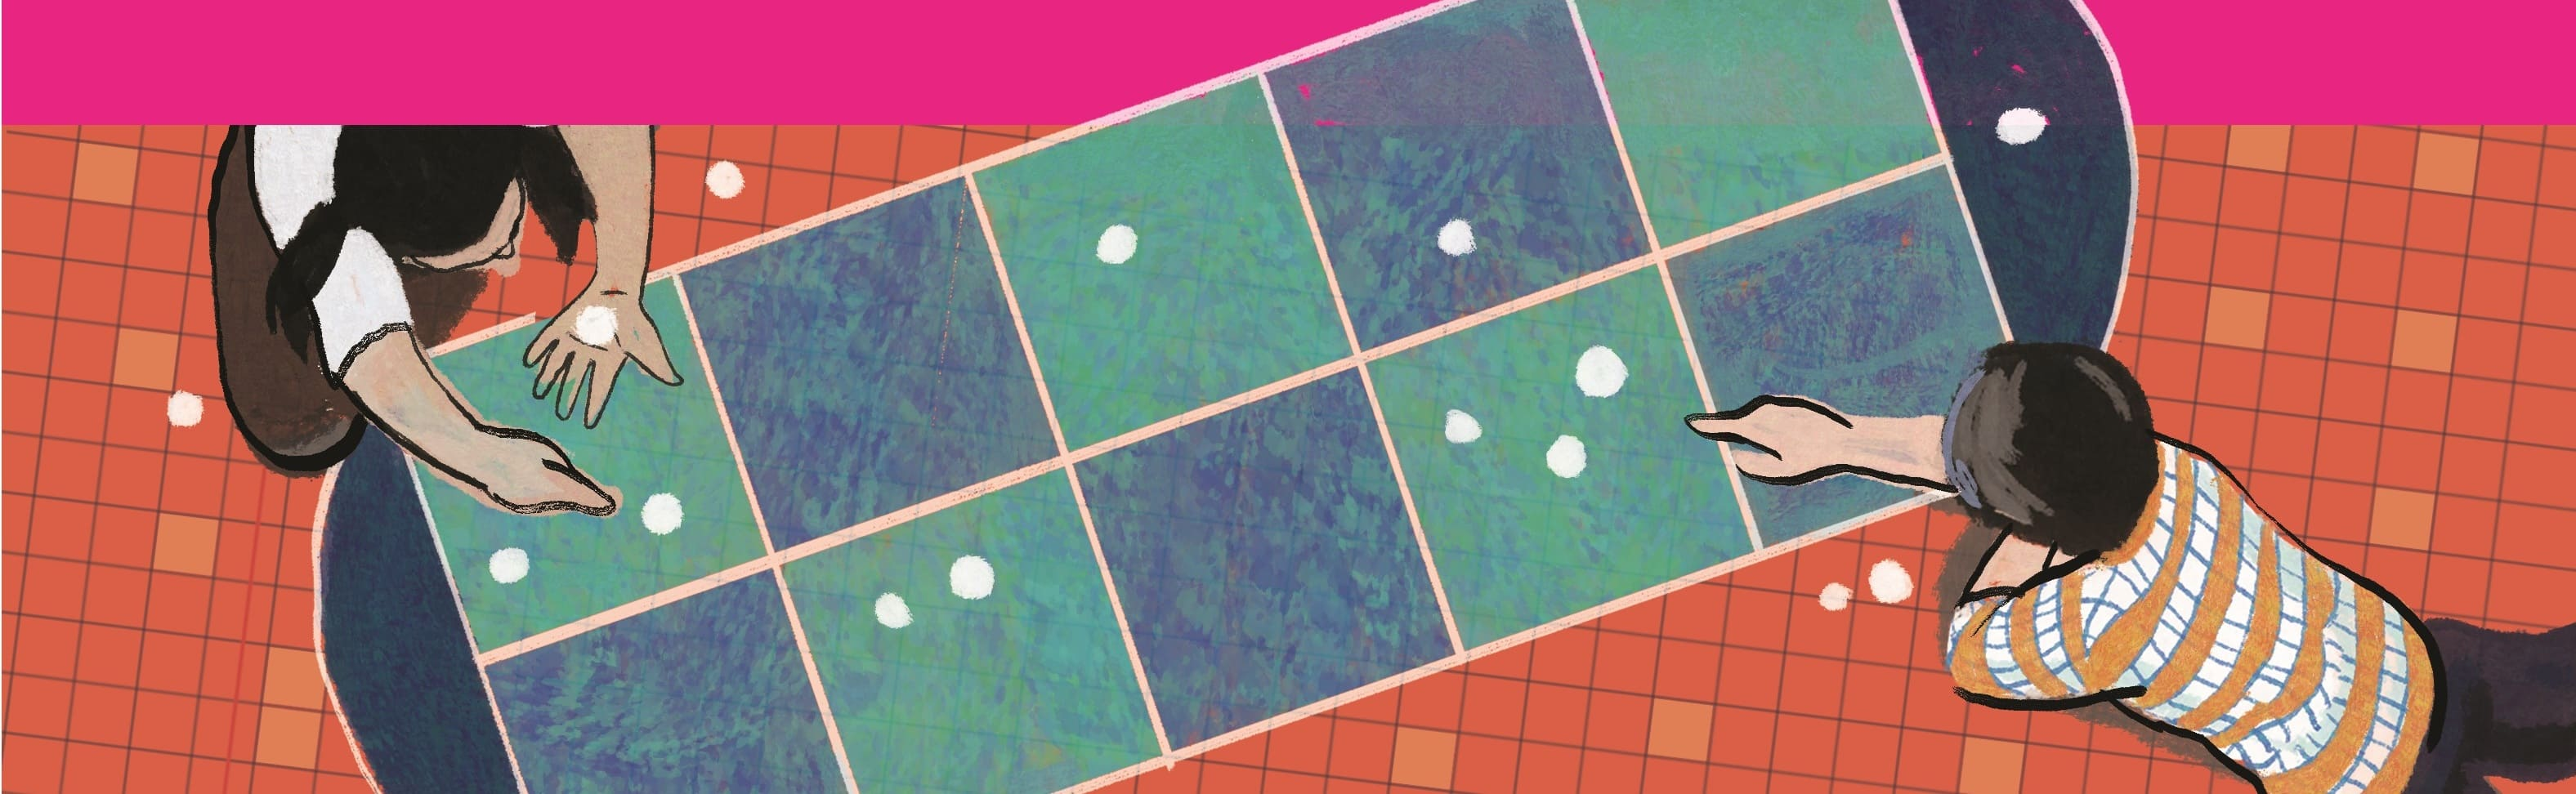
\includegraphics[width=19.3cm]{../bannertoancuabi}}}  
\AddToShipoutPicture*{\put(90,555){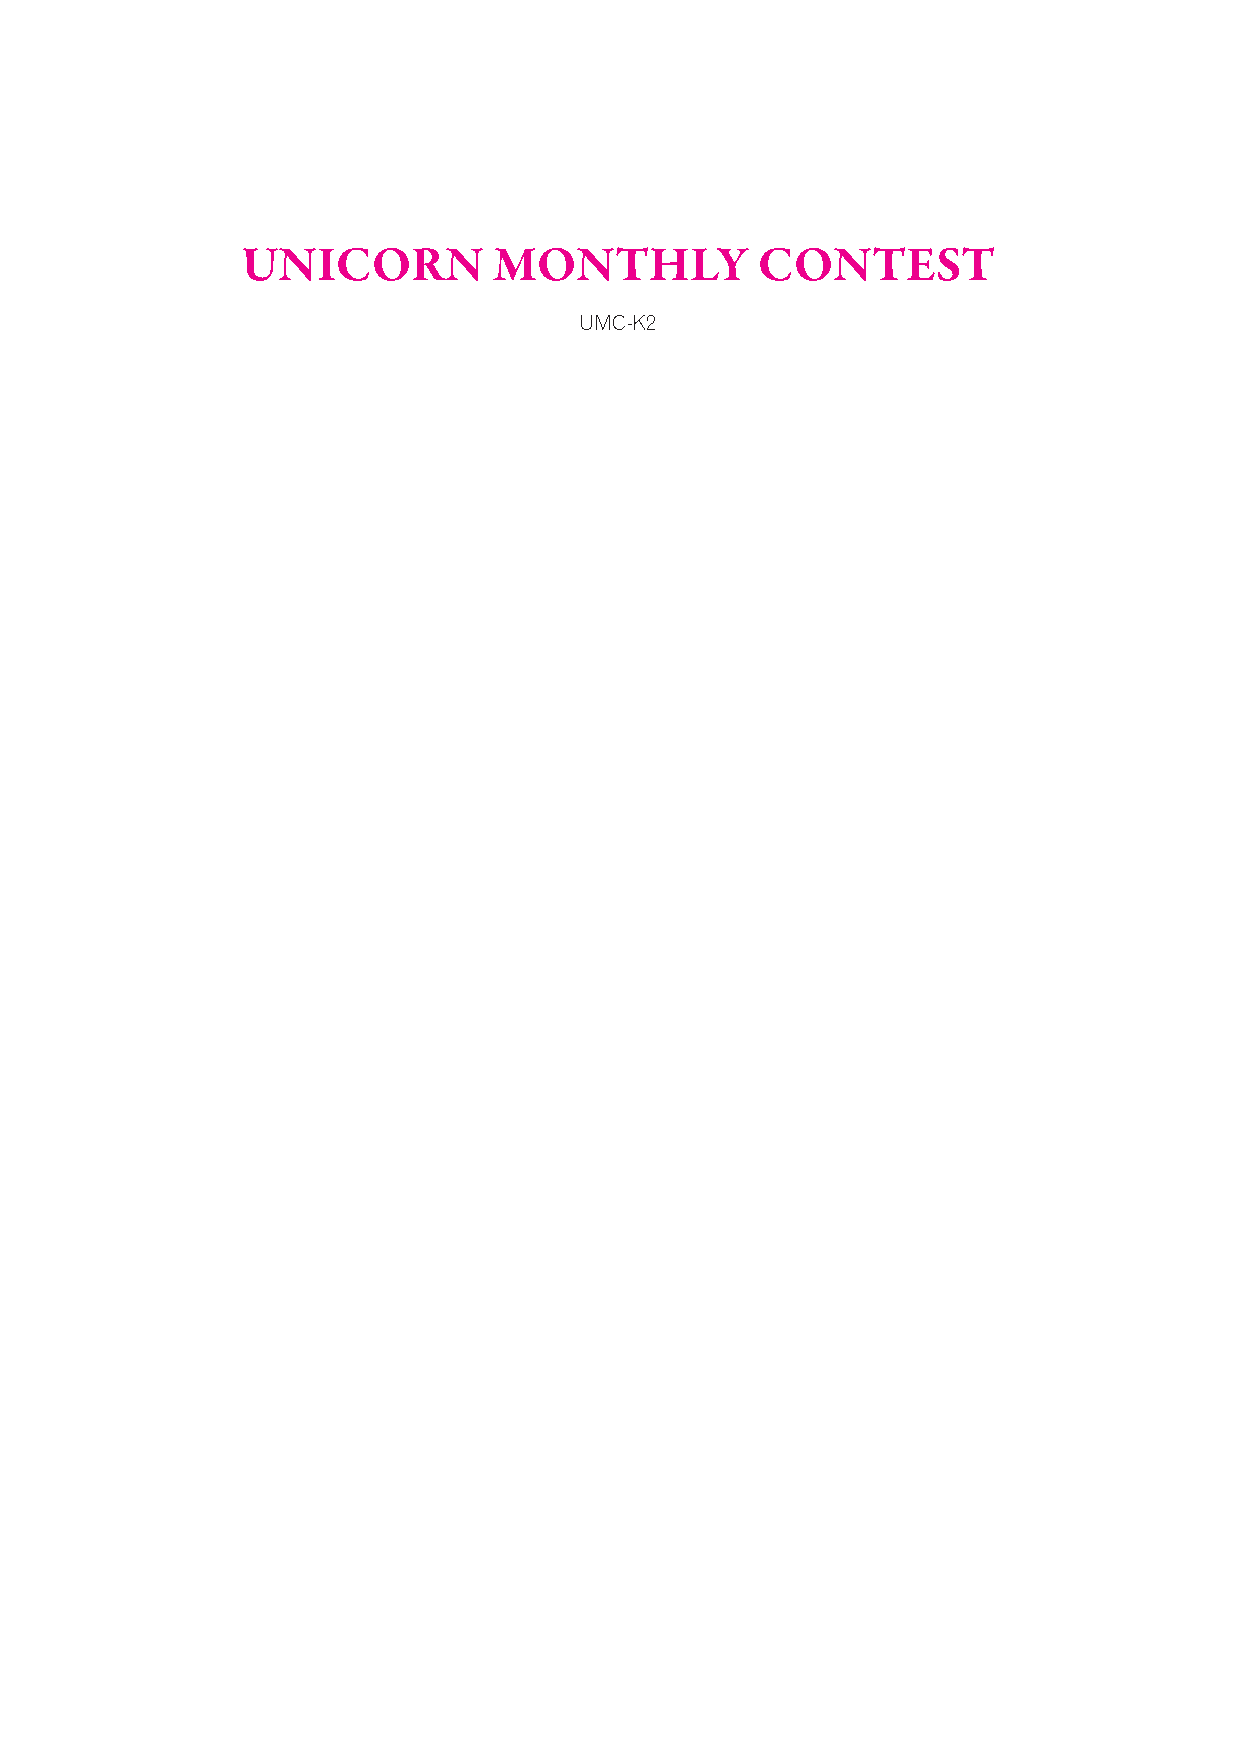
\includegraphics[scale=1]{../tieude1b.pdf}}} 
\centering
\endgroup
\vspace*{155pt}

\begin{multicols}{2}
	\textbf{\color{toancuabi}Bài} $\pmb{1.}$ Con chim nào cần bay ra khỏi ô vuông để mỗi hàng, mỗi cột có đúng $2$ con chim?
	\begin{figure}[H]
		\vspace*{-5pt}
		\centering
		\captionsetup{labelformat= empty, justification=centering}
		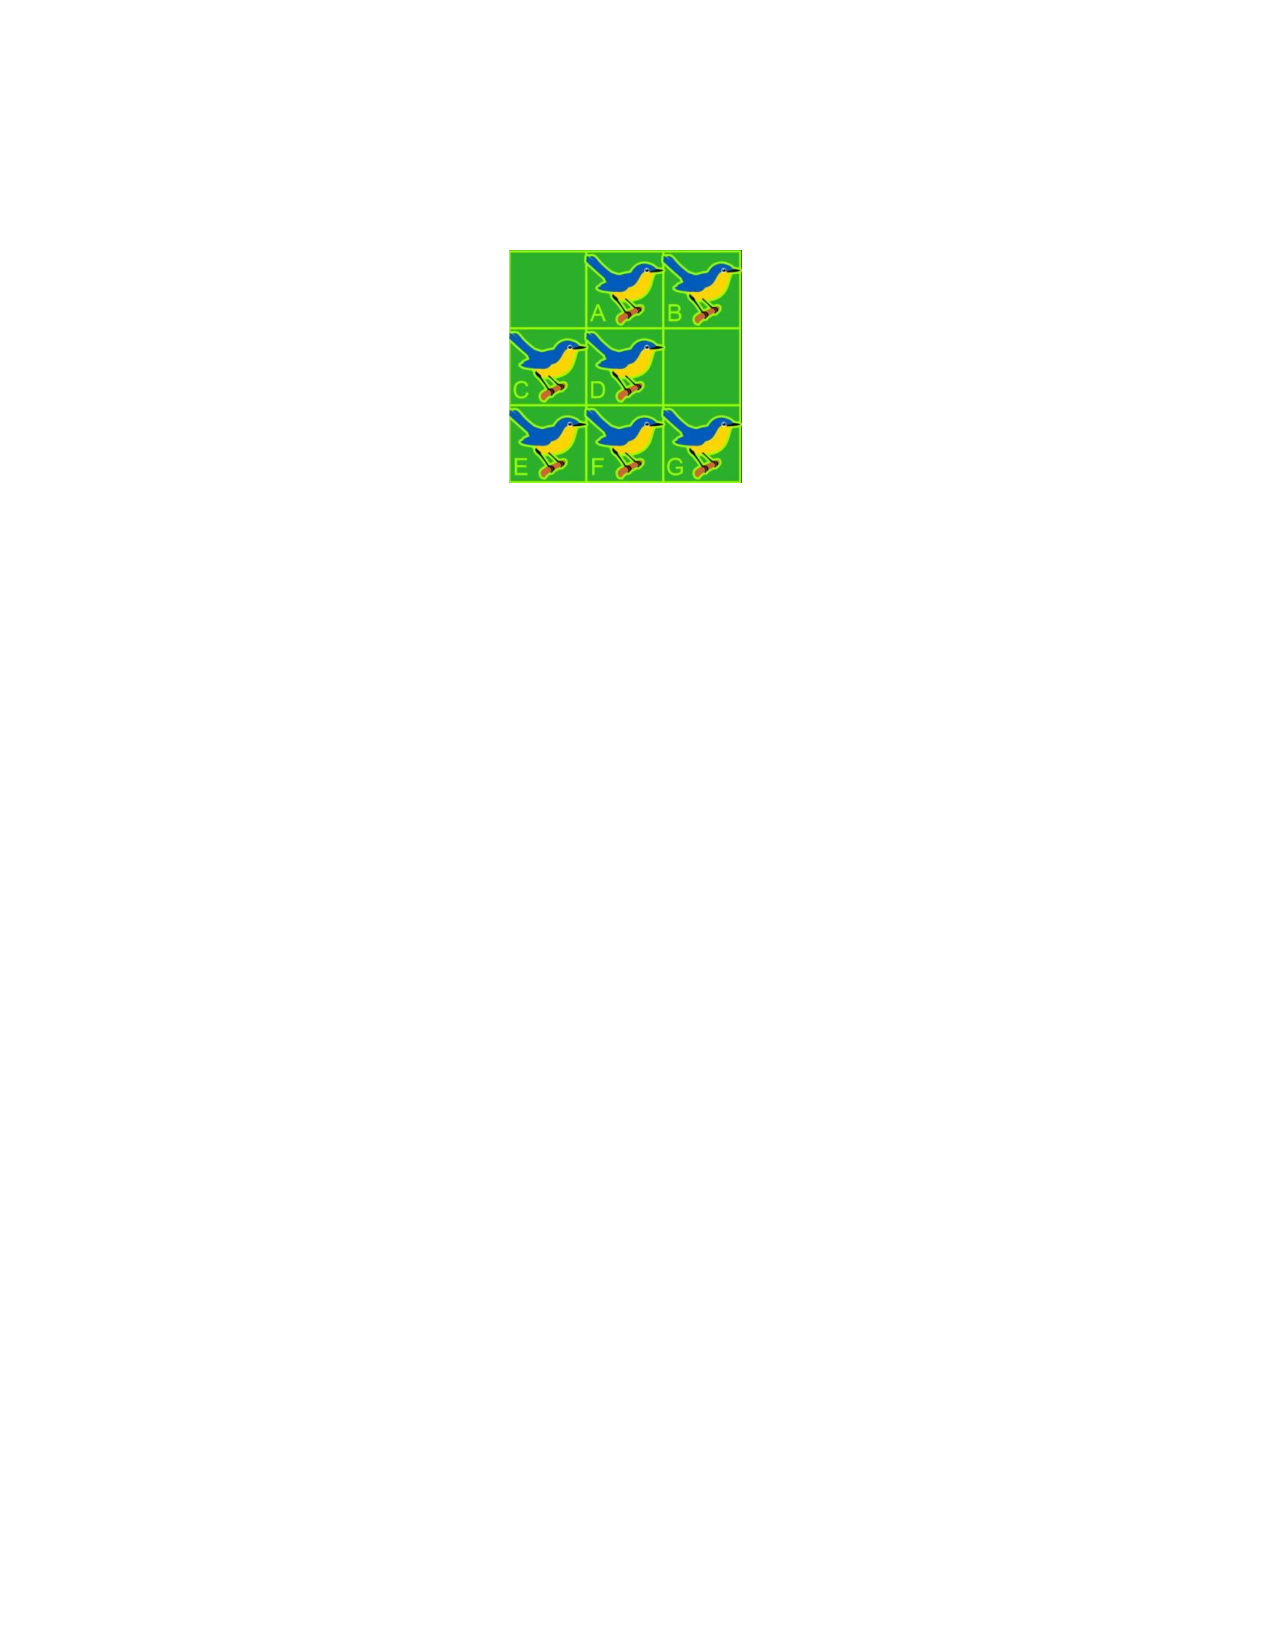
\includegraphics[width= 0.7\linewidth]{bai1k3}
		\vspace*{-10pt}
	\end{figure}
	\textbf{\color{toancuabi}Bài} $\pmb{2.}$ Có bao nhiêu đoạn thẳng trên hình vẽ bên.
	\begin{figure}[H]
		\vspace*{-5pt}
		\centering
		\captionsetup{labelformat= empty, justification=centering}
		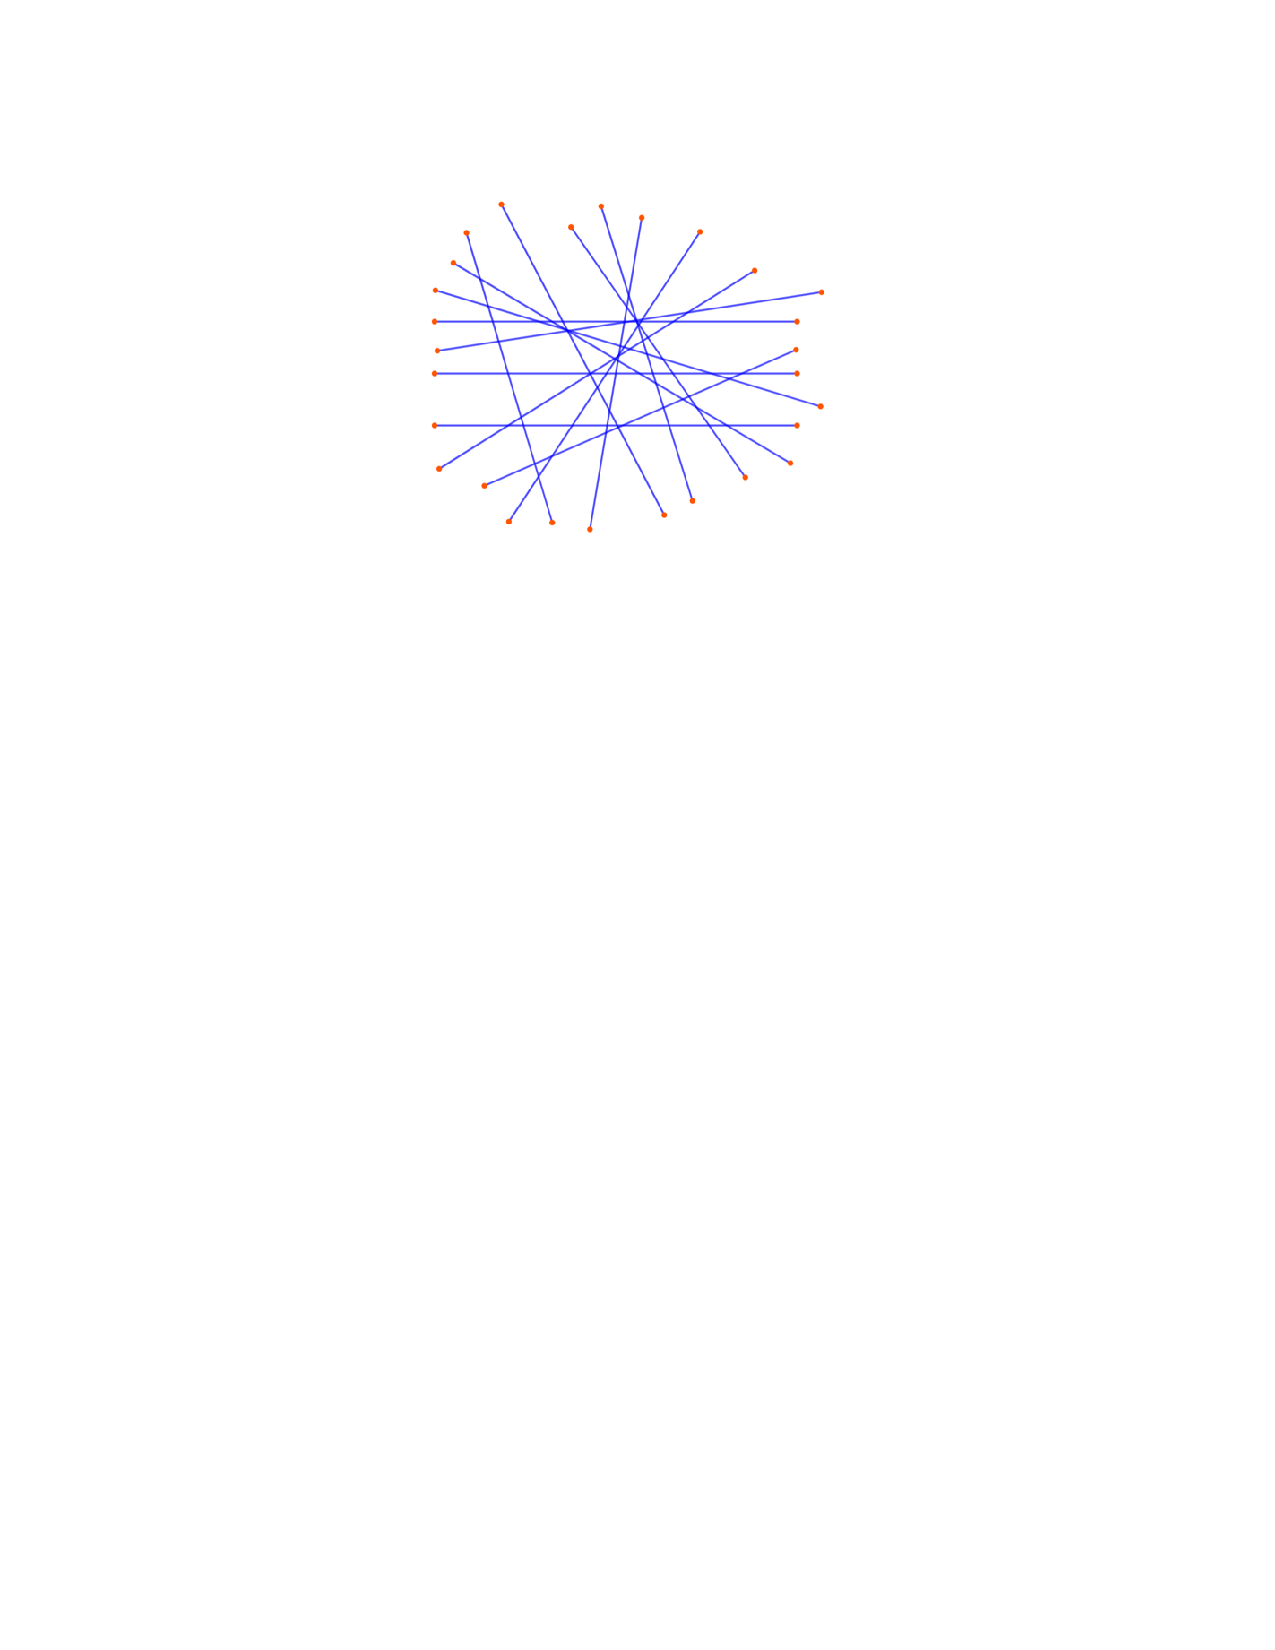
\includegraphics[width= 0.75\linewidth]{bai2k3}
		\vspace*{-5pt}
	\end{figure}
	\textbf{\color{toancuabi}Bài} $\pmb{3.}$ Hình lập phương bên trái trải ra thành hình bên phải. Hỏi trong ô hình $\nabla$ là số mấy?
	\begin{figure}[H]
		\vspace*{-5pt}
		\centering
		\captionsetup{labelformat= empty, justification=centering}
		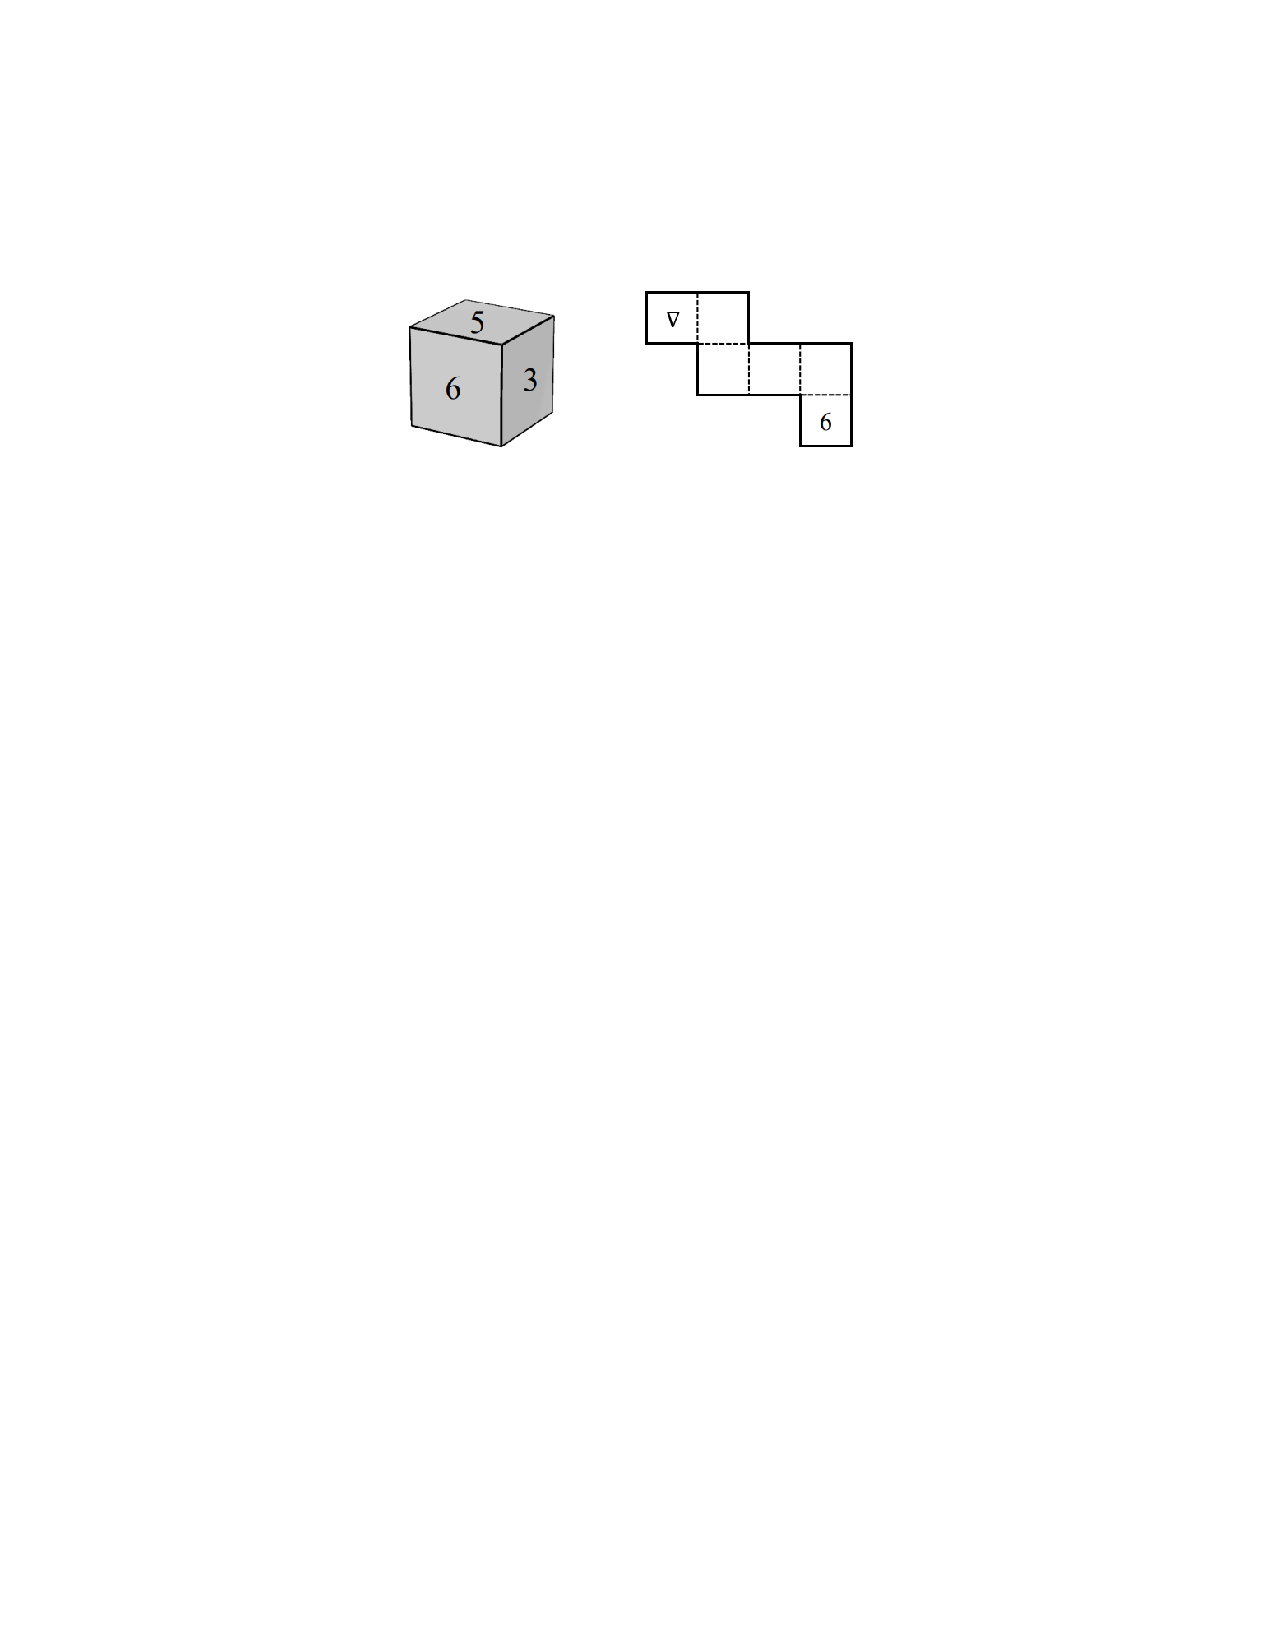
\includegraphics[width= 0.9\linewidth]{bai3k3}
		\vspace*{-10pt}
	\end{figure}
	\textbf{\color{toancuabi}Bài} $\pmb{4.}$ Tìm số có $2$ chữ số $AB$ thỏa mãn điều kiện như
	phép tính bên.
	\begin{table}[H]
		\vspace*{-5pt}
		\centering
		\captionsetup{labelformat= empty, justification=centering}
		\begin{tabular}{ccc}
			&$A$&$B$\\
			$\times$& &$A$\\
			\hline
			$B$&$A$&$A$\\
		\end{tabular}	
		\vspace*{-10pt}
	\end{table}
	\textbf{\color{toancuabi}Bài} $\pmb{5.}$ Hình bên có bao nhiêu hình vuông?
	\begin{figure}[H]
		\vspace*{-5pt}
		\centering
		\captionsetup{labelformat= empty, justification=centering}
		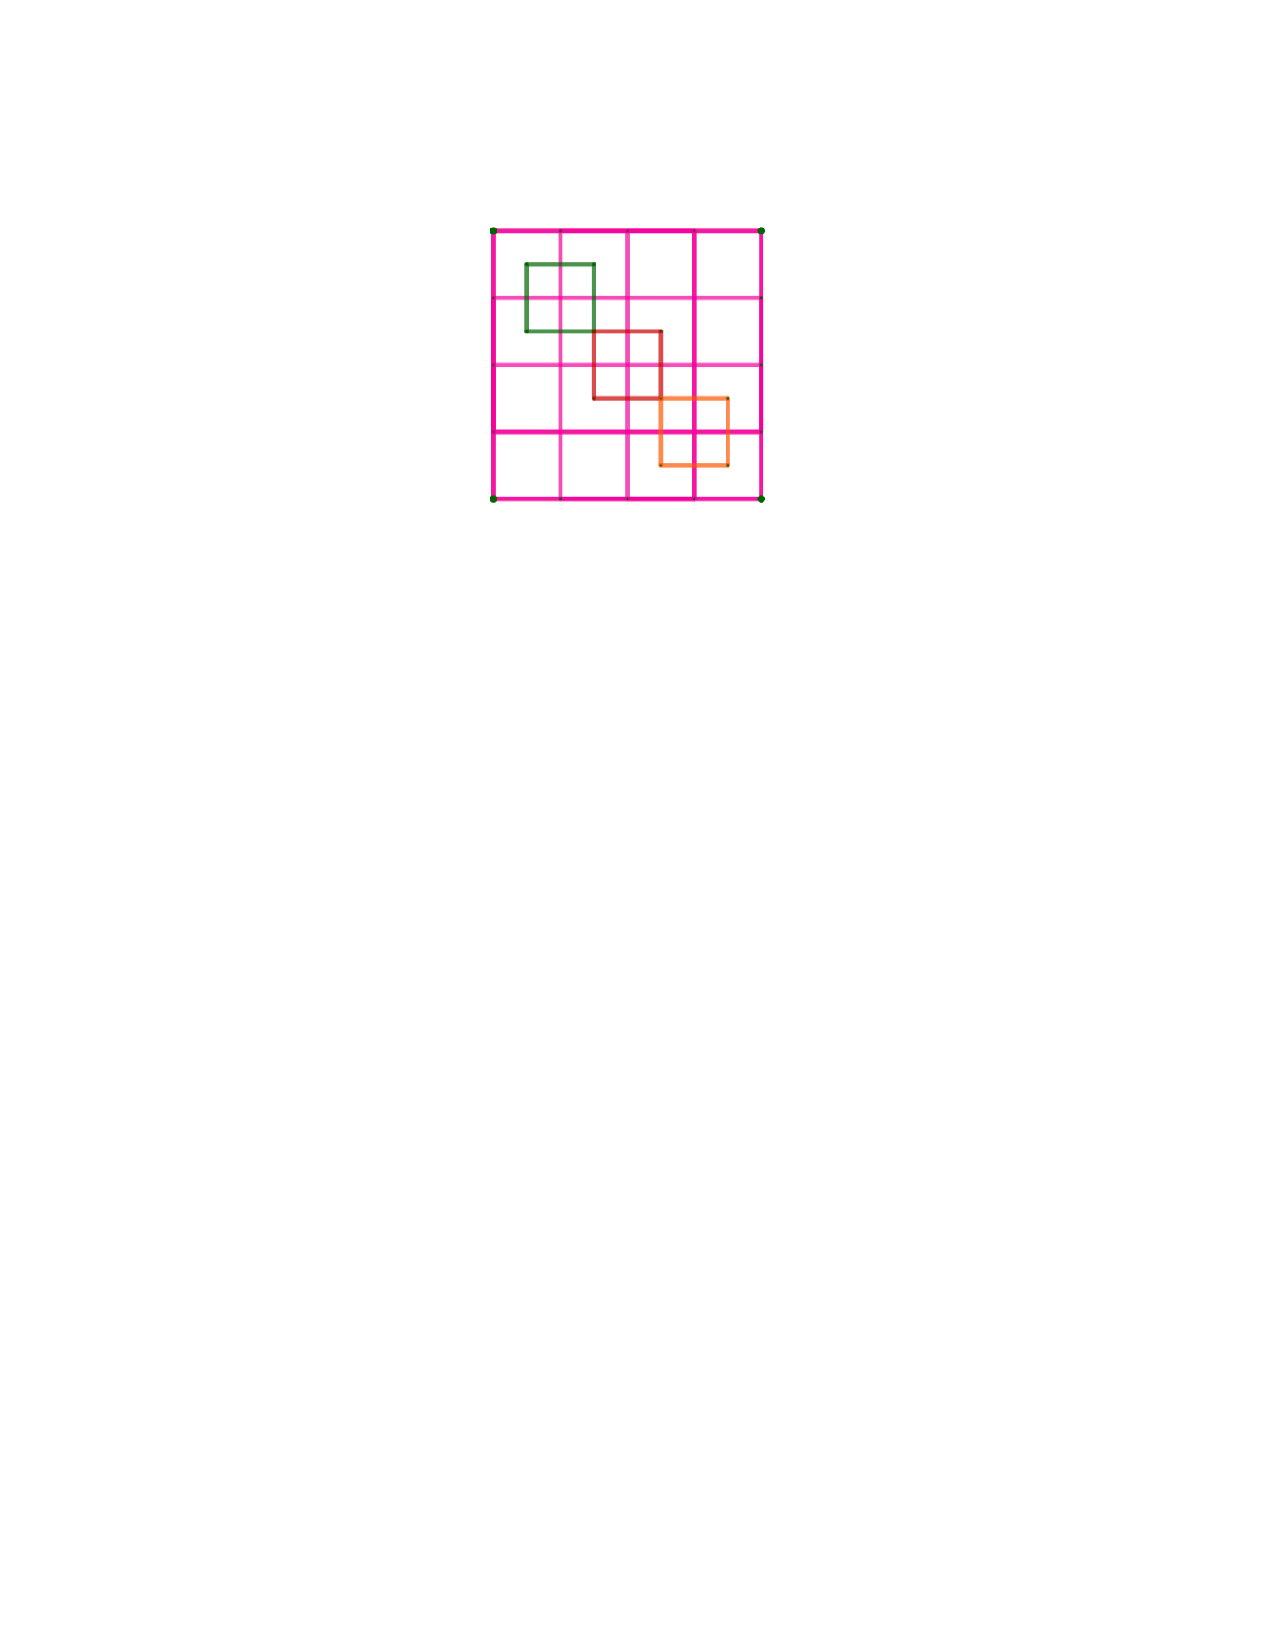
\includegraphics[width= 0.7\linewidth]{bai5k3}
		\vspace*{-10pt}
	\end{figure}
	\textbf{\color{toancuabi}Bài} $\pmb{6.}$ Số có $3$ chữ số ``dạng núi" là số có chữ số ở giữa lớn hơn $2$ chữ số bên cạnh nó. Có bao nhiêu số có $3$ chữ số dạng núi?
	\vskip 0.1cm
	\textbf{\color{toancuabi}Bài} $\pmb{7.}$ Điền số thích hợp vào chỗ trống:
	\begin{align*}
		135, 791, 113, 151, \_\_\_
	\end{align*}
	\textbf{\color{toancuabi}Bài} $\pmb{8.}$ Trên bảng ghi $21$ số chẵn liên tiếp. Bạn Phong xóa đi $1$ số và thấy tổng của các số còn lại bằng $2024$. Hỏi Phong đã đi xóa đi số nào?
	\vskip 0.1cm
	\textbf{\color{toancuabi}Bài} $\pmb{9.}$ Trong một cái túi có chứa các viên bi có bốn màu khác nhau: xanh, đỏ, tím, vàng. Cần phải lấy một cách ngẫu nhiên từ trong túi ra ít nhất bao nhiêu bi để chắc chắn có $3$ bi cùng màu nằm trong số
	đó?
	\vskip 0.1cm
	\textbf{\color{toancuabi}Bài} $\pmb{10.}$ Hai tam giác đều $ABC$ và $MNP$ có
	các cạnh tương ứng song song với nhau, tam giác $ABC$ có $3$ cạnh tiếp xúc với đường tròn tâm $O$ và tam giác $MNP$ có $3$ đỉnh nằm trên đường tròn đó. Biết diện tích tam giác $ABC$ bằng $60$ cm$^2$. Tam giác $MNP$ có diện tích
	bằng bao nhiêu cm$^2$?
	\begin{figure}[H]
		\vspace*{-5pt}
		\centering
		\captionsetup{labelformat= empty, justification=centering}
		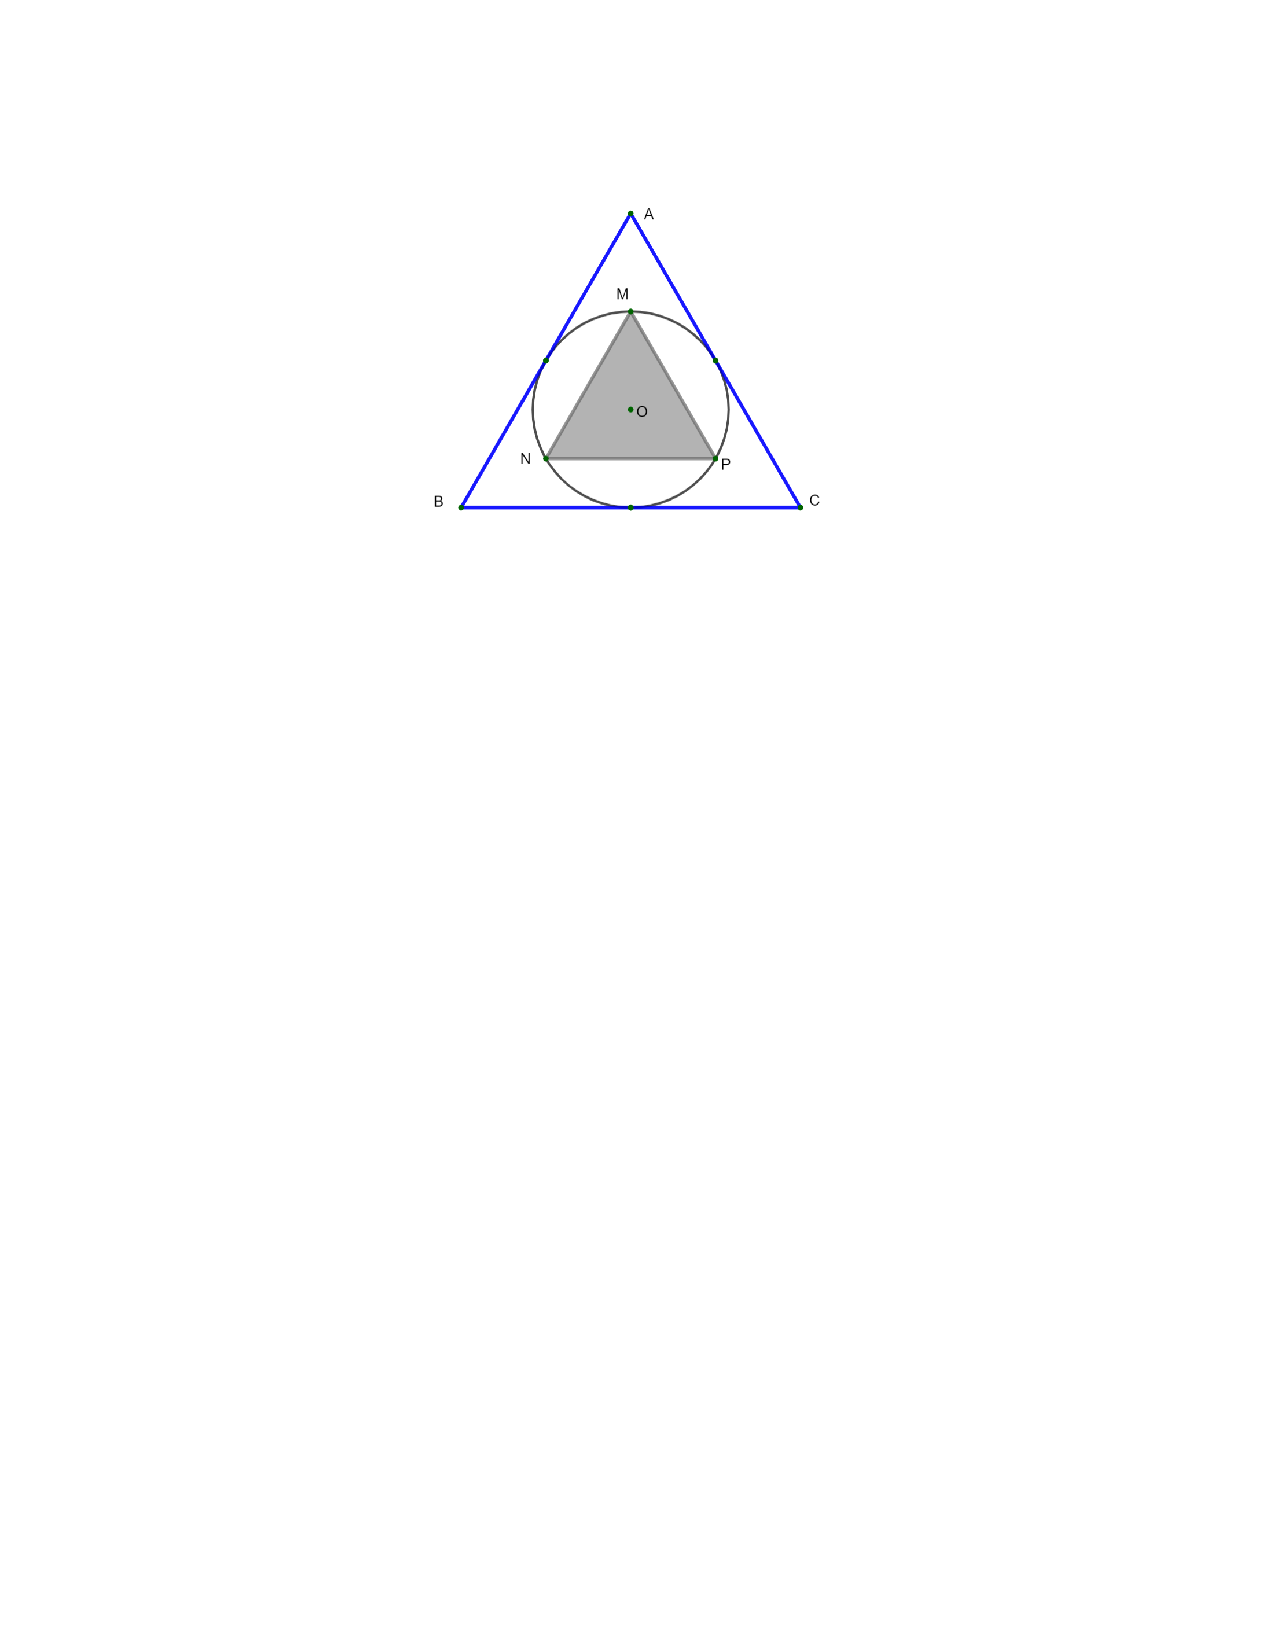
\includegraphics[width= 0.7\linewidth]{bai10k2}
		\vspace*{-10pt}
	\end{figure}
	\textbf{\color{toancuabi}Bài} $\pmb{11.}$ Có $15$ bạn nhỏ vào rừng hái nấm, không có $2$ bạn nào hái được cùng số nấm. Hỏi các bạn cần hái nhiều nhất bao nhiêu cái nấm để chắc chắn rằng có $2$ bạn hái được số nấm như nhau?
	\vskip 0.1cm
	\textbf{\color{toancuabi}Bài} $\pmb{12.}$ Một cái khóa số có mã gồm $3$ chữ số với các thông tin như hình bên. Bạn hãy phá khóa và cho biết mã của khóa là số nào?
	\begin{figure}[H]
		\vspace*{-5pt}
		\centering
		\captionsetup{labelformat= empty, justification=centering}
		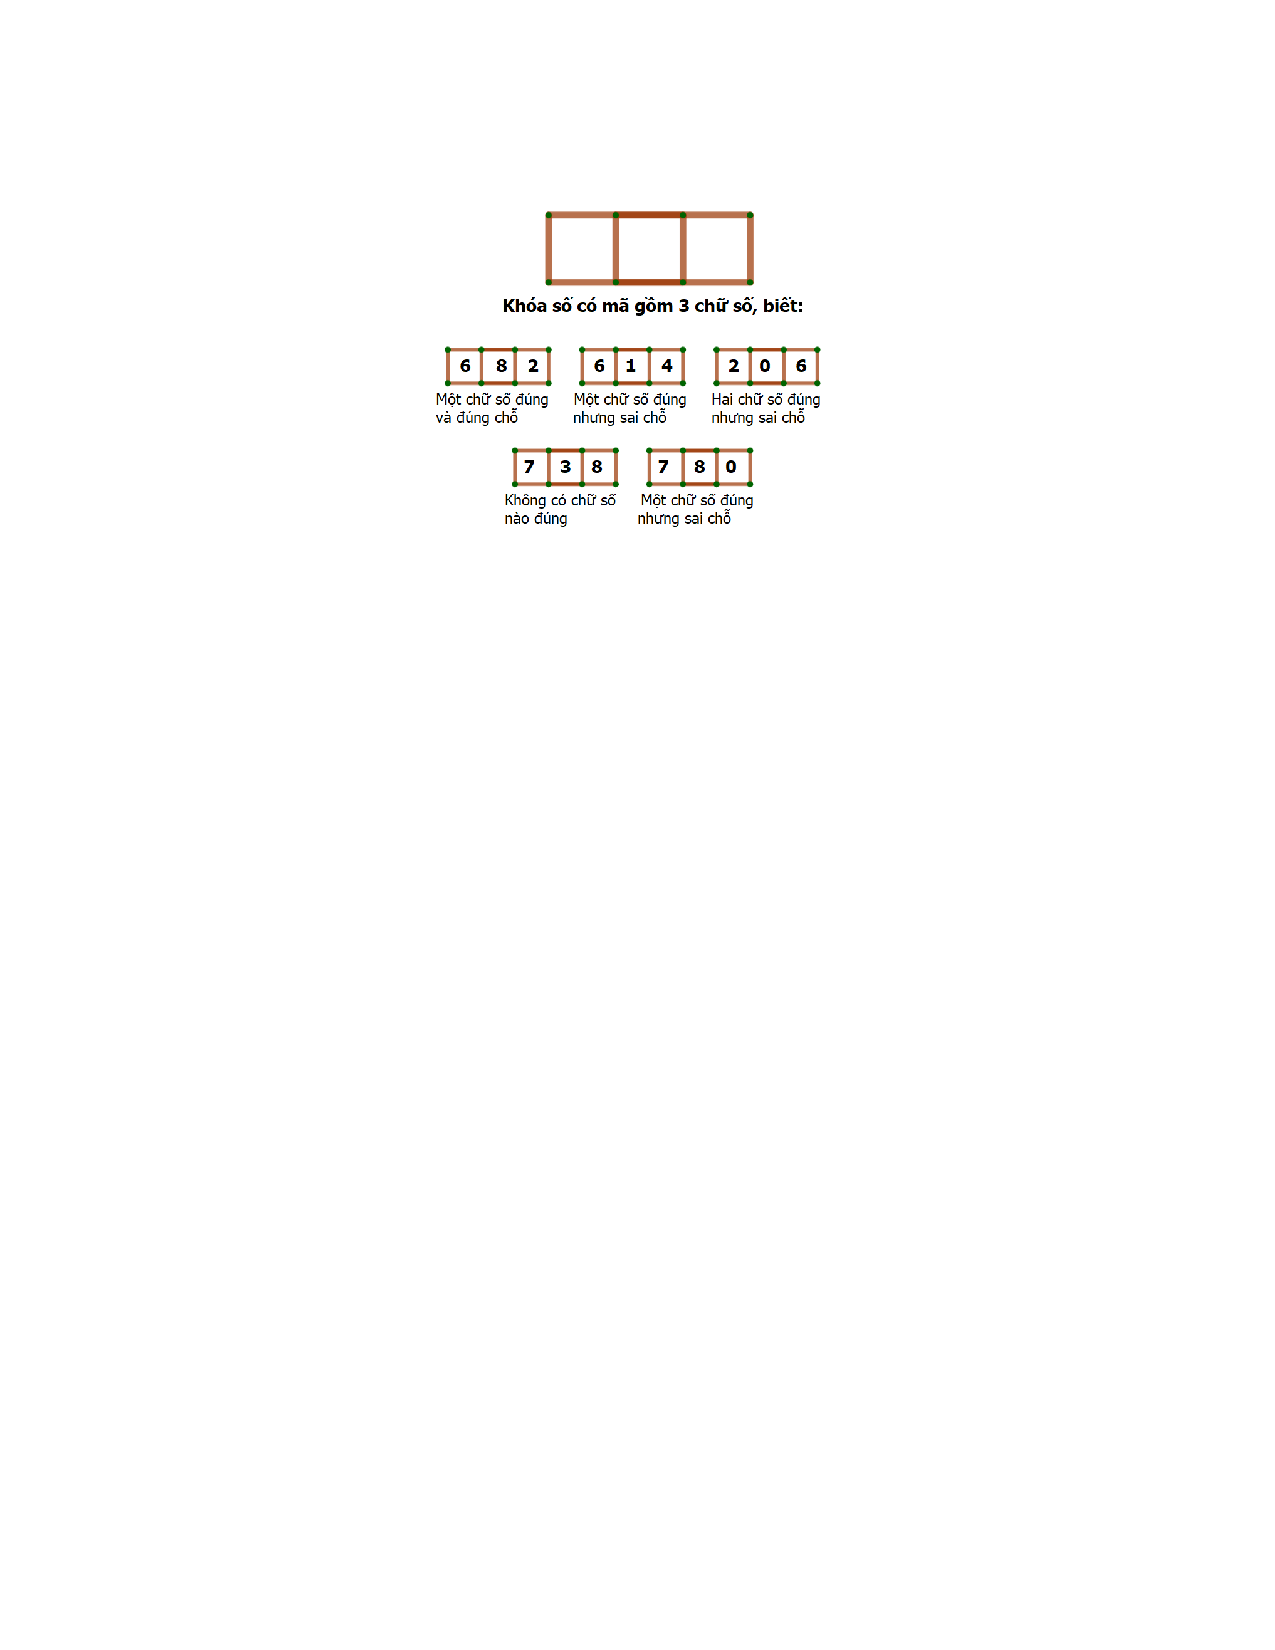
\includegraphics[width= 1\linewidth]{bai12}
		\vspace*{-15pt}
	\end{figure}
	\textbf{\color{toancuabi}Bài} $\pmb{13.}$ Tính giá trị của $S$.
	\begin{align*}
		S =& \frac{1}{1\times 2 \times 5} + \frac{1}{2\times 5 \times 6} + \frac{1}{6\times9\times 10} \\
		&+ \cdots + \frac{1}{26 \times 29 \times 30} + \frac{1}{29\times 30 \times 33}
	\end{align*}
	\textbf{\color{toancuabi}Bài} $\pmb{14.}$  Xác định số phù hợp ở ô tròn trống.
	\begin{figure}[H]
		\vspace*{-5pt}
		\centering
		\captionsetup{labelformat= empty, justification=centering}
		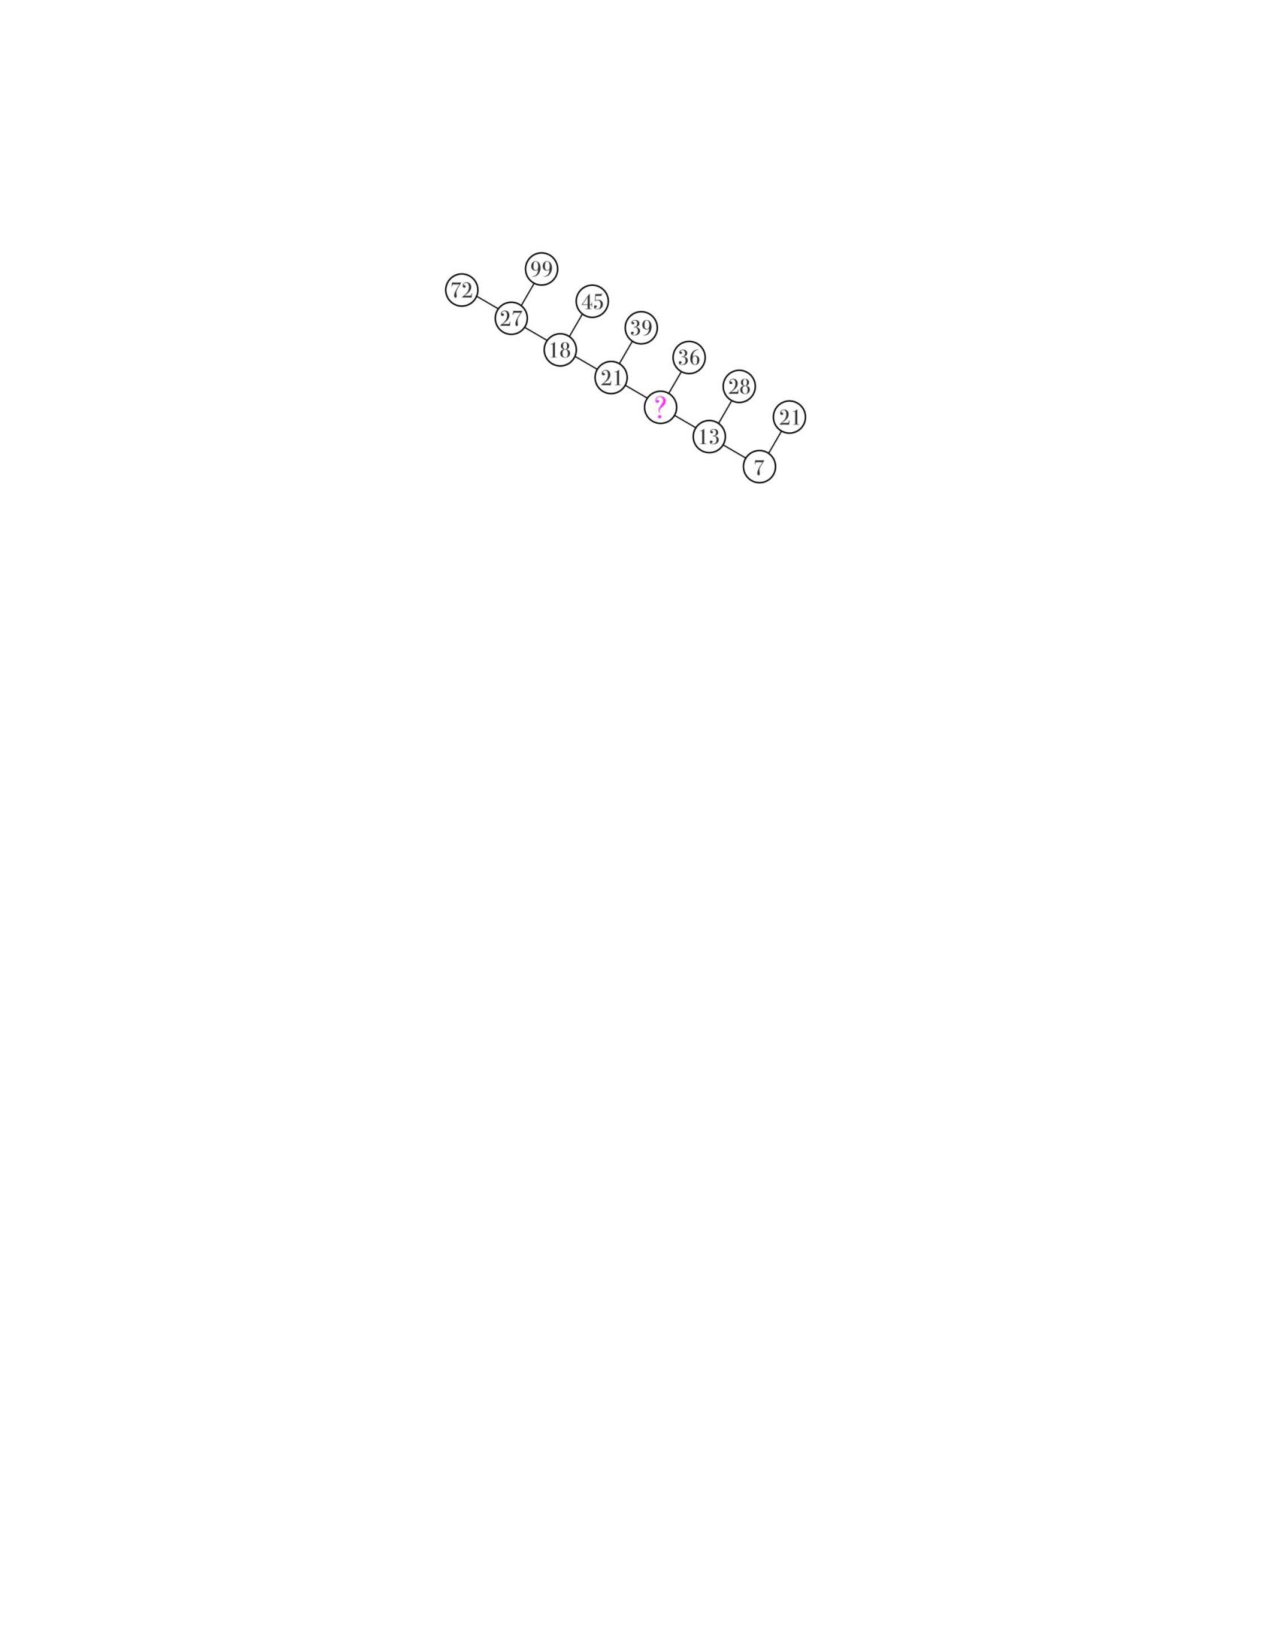
\includegraphics[width= 1\linewidth]{bai14k3}
		\vspace*{-10pt}
	\end{figure}
	\textbf{\color{toancuabi}Bài} $\pmb{15.}$ Có bao nhiêu cách chọn ra $2$ số từ các số trong tập hợp $S=\{1,2,3,4,..,19,20\}$ sao cho tích của chúng là số chẵn?
	\vskip 0.1cm
	\textbf{\color{toancuabi}Bài} $\pmb{16.}$  Một số có ba chữ số được viết ngẫu nhiên. Xác suất để tổng các chữ số của số này bằng $5$ là bao nhiêu? (Viết kết quả dưới dạng phân số tối giản)
	\vskip 0.1cm
	\textbf{\color{toancuabi}Bài} $\pmb{17.}$  Có bao nhiêu cách tô màu $4$ miền $A,B,C,D$ như hình vẽ bằng các màu Xanh, Đỏ, Vàng (không nhất thiết dùng cả $3$ màu) sao cho không có $2$ miền nào kề nhau có cùng màu.
	\vskip 0.1cm
	\textit{(Hai miền kề nhau là hai miền có chung cạnh).}
	\vskip 0.1cm
	\textbf{\color{toancuabi}Bài} $\pmb{18.}$ Hình vuông ma thuật $3\times 3$ có tổng các hàng, các cột và $2$ đường chéo đều bằng nhau. Hình bên là một hình vuông ma thuật. Tìm giá trị của $a$?
	\begin{figure}[H]
		\vspace*{-5pt}
		\centering
		\captionsetup{labelformat= empty, justification=centering}
		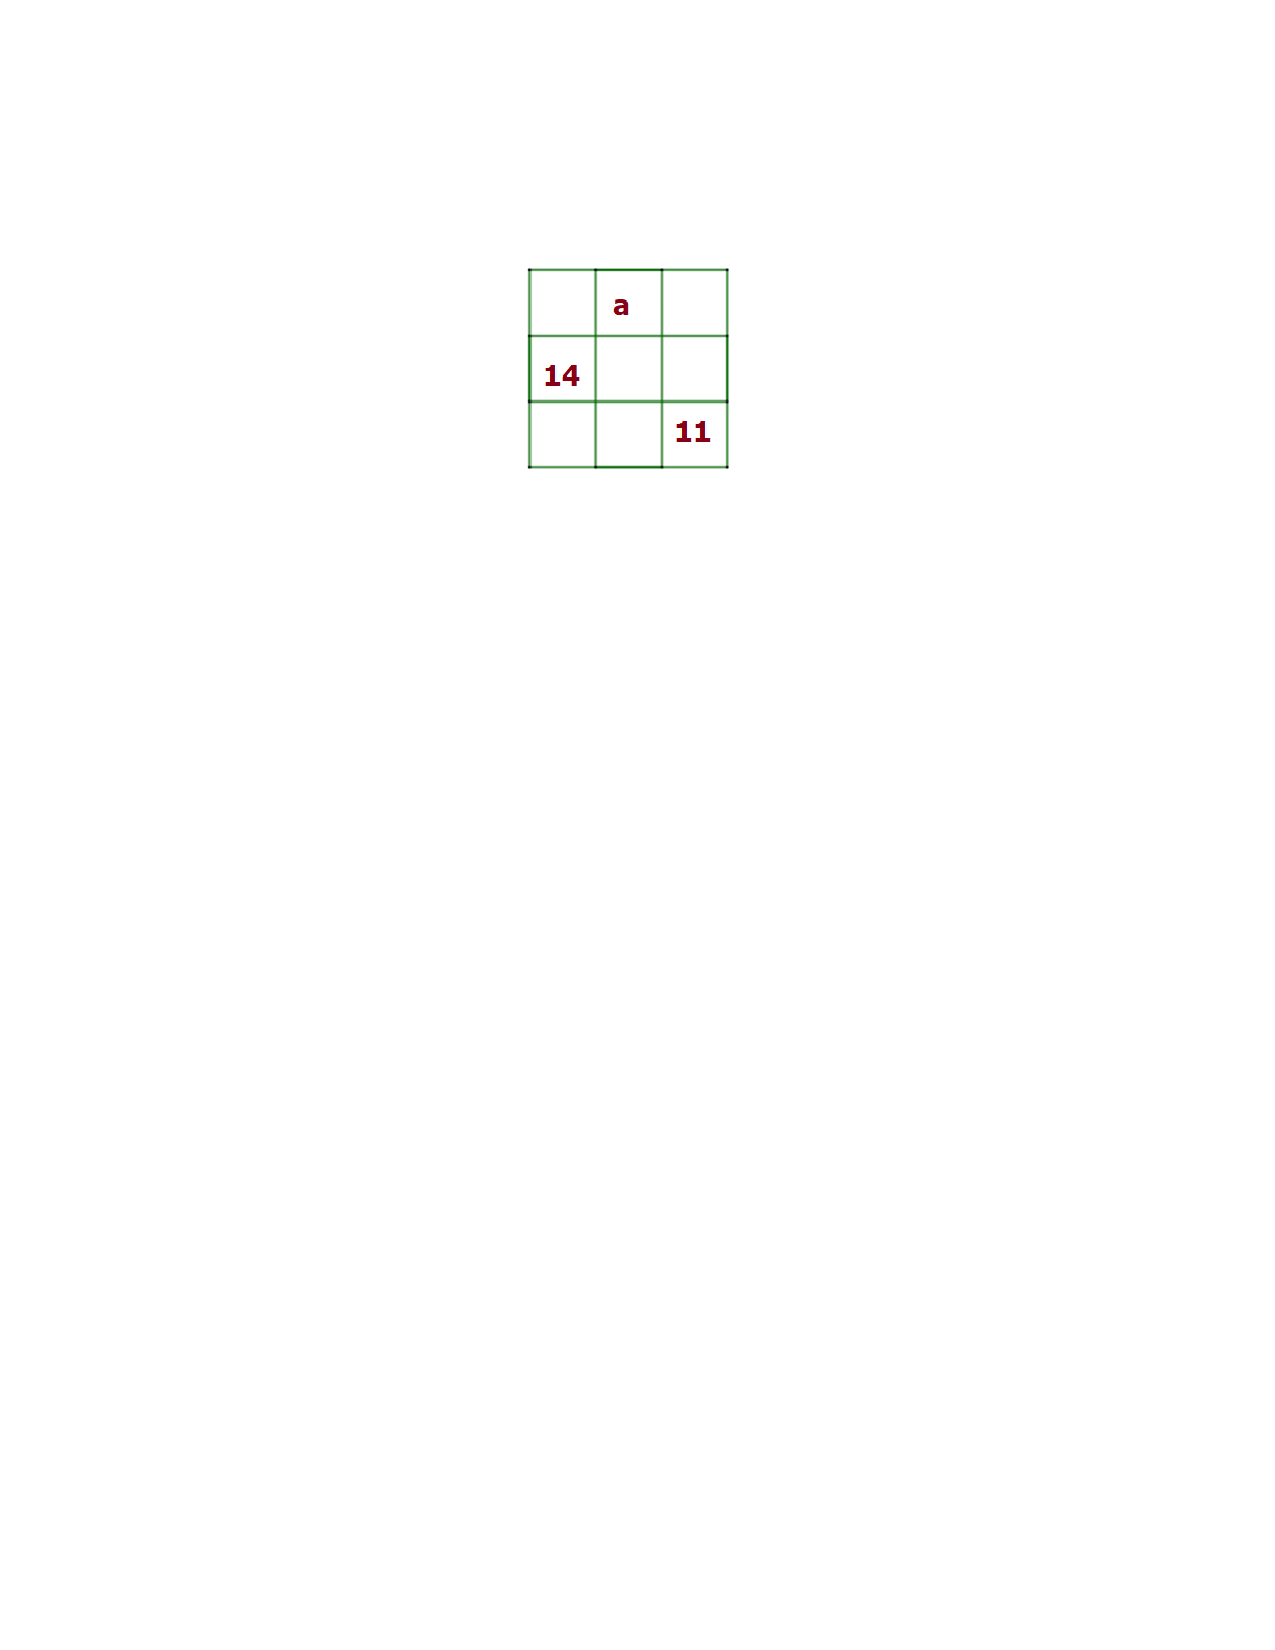
\includegraphics[width= 0.7\linewidth]{bai18k3}
		\vspace*{-10pt}
	\end{figure}
	\textbf{\color{toancuabi}Bài} $\pmb{19.}$  Ba số được chọn ngẫu nhiên từ $10$ số $\{1,2,3,..,10\}$. Xác suất để tổng ba số này chia hết cho $3$ là bao nhiêu?
	\vskip 0.1cm
	\textbf{\color{toancuabi}Bài} $\pmb{20.}$ Có bao nhiêu cách để chia $6$ bạn $A,B,C,D,E,F$ thành $2$ đội, mỗi đội gồm $3$ bạn?
\end{multicols}